\exer{Détermination du nombre de bit de la mantisse d'un flottant}

On se propose de vérifier que le stockage de la mantisse d'un flottant \texttt{python} s'effectue sur 52 bits.
On note $m_c=m-1$, \texttt{m} étant la mantisse du flottant. \texttt{mc} est la valeur stockée en mémoire en binaire.
L'idée est de se servir du nombre $0,5$ dont on connait parfaitement la décomposition binaire :

\begin{center}
$0,5=\frac{1}{2}=1 \times \frac{1}{2} + 0 \times \frac{1}{4} + 0 \times \frac{1}{8}... $
\end{center}

On observe qu'en divisant $m_c$ successivement par 2 on obtient :
\begin{center}
$
\begin{array}{l l l l}
m_c=0.5 & m=1.5 & \mbox{stockée en mémoire sous la forme} & 1000...000\\
m_c=0.25 & m=1.25 & \mbox{stockée en mémoire sous la forme} & 0100...000\\
m_c=0.125 & m=1.125 & \mbox{stockée en mémoire sous la forme} & 0010...000\\
...\\
m_c=0.00...1 & m=1.00...1 & \mbox{stockée en mémoire sous la forme} & 0000...001\\
\end{array}
$
\end{center}

Au bout d'un nombre suffisamment grand de divisions par 2 le chiffre 1 disparait complètement. En comptant le nombre de divisions par 2 nécessaires pour aboutir à 0, on a accès au nombre de bits disponibles pour coder $m_c$.\\
On propose l'algorithme suivant :

\begin{tabular}{p{1cm}|p{1cm}|p{5cm}}
& \multicolumn{2}{l}{Initialisation (à compléter)} \\
& \multicolumn{2}{l}{\textbf{Tant que} $1+m_c \neq 1$ \textbf{faire}} \\
&& $m_c \leftarrow m_c/2 $\\
&& $i \leftarrow i+1 $\\
& \multicolumn{2}{l}{\textbf{fin}} \\
& \multicolumn{2}{l}{\textbf{retourner } $i$} \\
\end{tabular}


%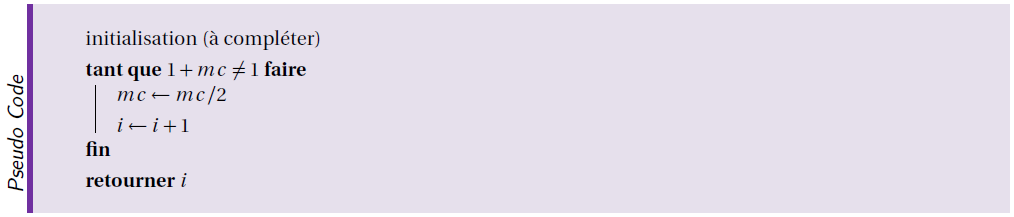
\includegraphics[scale=0.67]{pseudo.png}

\question{
Commenter ou compléter l'algorithme proposé :}
\vspace{-.5cm}
\textit{\begin{itemize}
\item compléter la partie initialisation;
\item justifier le type de boucle choisie;
\item repérer la condition d'arrêt;
\item invariant de boucle;
\item la boucle a-t-elle une fin ?
\item l'algorithme effectue t-il ce que l'on attend ?
\end{itemize}}



\question{Implémenter cet algorithme dans \texttt{python}. Conclure quant au nombre de bits disponibles pour coder la mantisse d'un flottant.}

Il est possible d'appliquer la méthode \texttt{hex()} sur un flottant pour avoir sa représentation en hexadécimal.

\begin{lstlisting}
>>> f = 5.25
>>> f.hex()
        '0x1.5000000000000p+2'
\end{lstlisting}

Cela dit que 5,25 est représentée par le nombre $1\times (5000000000000)_{16} \times 2^{2}$
dont la mantisse est 1,5000000000000 et l'exposant 2.
%\invite rad = 2.0 ** .5\\
%\invite rad.hex ()\\
%'0x1.6a09e667f3bcdp+0'
%La mantisse est 1.6a09e667f3bcdp et l'exposant 0

\question{Déterminer la mantisse de $\sqrt{2}$ à partir de son expression hexadécimale.}
